\item \textbf{Riemann sums can be used to estimate the area under the curve $y =f (x)$ in the interval $[a, b]$. Left-and right-endpoint approximations, with subintervals of the same width, are special kinds of Riemann sums, ie,
    \begin{center}
        Left-endpoint approximation:
    \end{center}
    \begin{equation*}
        L_n = \sum_{i=1}^n f(x_{i-1})\Delta x
    \end{equation*}
    \begin{center}
        Right-endpoint approximation:
    \end{center}
    \begin{equation*}
        R_n = \sum_{i=1}^n f(x_{i})\Delta x
    \end{equation*}
    \begin{equation*}
        \text{where} \; \Delta x = \frac{b-a}{n} \qquad x_i=a+i\Delta x, \; i=0,1,\cdots,n
    \end{equation*}
    Implement functions to compute L\textsubscript{n} and R\textsubscript{n} . Using the function $f (x) =sin x$ over the interval $[0, \frac{\pi}{2} ]$, compute L\textsubscript{n} and R\textsubscript{n} for n=10. Compare the previous results with
    \begin{equation*}
        \int\limits_{0}^{\frac{\pi}{2}} f(x)dx
    \end{equation*}
}

El programa que emplea los dos algoritmos se encuentra en la carpeta \textcolor{citecolor}{Problema\_4}. Los resultados de cada integral se muestran en la tabla \ref{table:resultados4} y el programa arroja los resultados en la terminal como se muestra en la figura \ref{fig:resultados4}.
\begin{figure}[H]
    \centering
    \includegraphics[width=8cm]{Graphics/problema4_ss.png}
    \caption{Resultados impresos en la termianl obtenidos por el programa}
    \label{fig:resultados4}
\end{figure}
En la figura \ref{fig:integracion} se muestra la representación gráfica de los algoritmos Left-endpoint y Right-endpoint.
\begin{figure}[H]
    \centering
    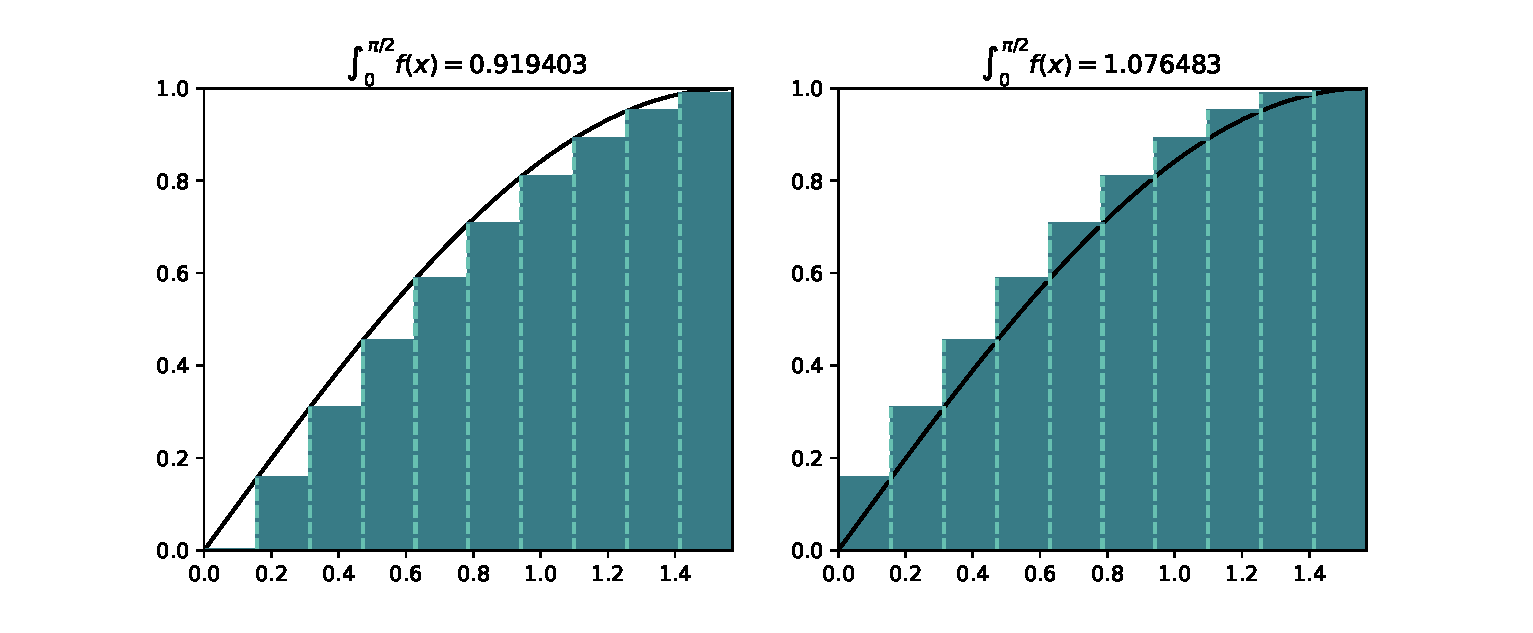
\includegraphics[width=17cm]{Graphics/integration.eps}
    \caption{Representación gráfica de los algoritmos left-endpoint (izquierda) y right-endpoint (derecha).}
    \label{fig:integracion}
\end{figure}
La diferencia obtenida entre los dos algoritmos de integración es de 0.157080.
\begin{table}[H]
    \centering
    \begin{tabular}{lc} \hline
        \textbf{Algoritmo} & \textbf{Resultado} \\\hline
        Left-endpoint      & 0.919403           \\
        Right-endpoint     & 1.076483           \\ \hline
    \end{tabular}
    \caption{Resultados de los algoritmos de integración con los parámetros especificados para $f(x)=sin(x)$}
    \label{table:resultados4}
\end{table}